\chapter{\textit{Kernel}-Based Nonlinear Spatial Transformation}\label{ch:spheremapping}
\section{Introduction}\label{sec:intro-kernel}

As discussed in Chapter 2, the main objective of the personalized classifier is to reassess the normal samples to identify deviation of seemingly normal samples into any of abnormality types. \textcolor{black}{The original geometry of clusters in the feature space $\Omega^d$ depends on the choice of features implied by the feature extraction and feature selection stages $g()$}. We noticed that with the resulting features (in this work), the clustering geometry does no exhibit the necessary symmetric property and thus leads to a poor performance and even failure in predicting subsequent abnormalities. 
Therefore, an optimization method based on spatial transformation is proposed to solve this issue. More specifically, we propose a method to reshape the clusters such that 
 \begin{itemize}
\item The abnormal classes surround the normal class; 
\item A maximal separation among the abnormal classes are achieved; 
\item The angles between the vectors connecting the centroid of normal cluster to different abnormal clusters are equalized. 
\end{itemize}

These properties can be achieved through imposing the following conditions:  
 \begin{itemize}
     %\item Vectors pointing from normal centroid to different abnormal clusters centroids has no overlapping or cross with each other.
     \item Vectors pointing from the normal centroid to different abnormal clusters centroids present maximum mutual cosine distances.
     \item The overlapping parts among all clusters are minimized.
 \end{itemize}

% maximizing the minimum of the angles between the aforementioned vectors from the normal cluster centroid to abnormal cluster centroids. 


Given that the clusters in original feature space do not meet these symmetric properties, developing a spatial transformation is unavoidable. In this chapter, a \textit{kernel}-based nonlinear spatial transformation is proposed to reshape the feature space to reach the above-mentioned required symmetric properties. 
%Here, we assume in this chapter that new feature space obtained by non-linear reshaping is noted as $\Phi^{d'}$. 
\textcolor{black}{This reshaping process is part of the \textcolor{black}{\textit{personalized classification}} stage (as shown in Fig.\ref{fig:flow}) of the ECG classification system as described in chapter 2. The nonlinear mapping projects the corresponding feature vector of each sample $\mathbf{x}_k$  in the original space $\Omega^d$ onto a new vector $\mathbf{z}_k$ in a higher dimensional space denoted by $\Omega^{d^\prime}$.  This is achieved using a nonlinear mapping function $\Psi^{d'}:\Omega^{d} \rightarrow \Omega^{d^\prime}$. The resulting vectors are used by the personalized classifier to identify the minor yellow alarm type out of $\{\mathcal{S},\mathcal{V},\mathcal{F}\}$.} 
%\textcolor{red}{
%The original text was ambiguous. Firstly, set and cluster shapes can be viewed differently, sets are not changes under the transformation although cluster geometry changes. Therefore, since we already used $\mathcal{N},...$ to represent clusters in the original space, you can use $\mathcal{N'},....$ for the transformed clusters, unless you mean a set (not a cluster). In this case, sets do not changes under the transformation, and you can omit the definition $\Phi^{d'}=\{\mathcal{N},\mathcal{S},\mathcal{V},\mathcal{F}\}$ to avoid ambiguity.
%Secondly, you need to distinguish between two functions, one simply maps the vector in original space into a new space, and the second one processes the transformed vector and maps it to a yellow alarm. It is not clear in the text.}

%  which can be considered as the union of subspaces for transferred types: %$\Phi^{d'}=\{\mathcal{N},\mathcal{S},\mathcal{V},\mathcal{F}\}$, where $d'>d$. 
  

\section{\textit{Kernel} Method}

Kernel method has been widely used in machine learning algorithms. For instance, it is the integral part of nonlinear Support Vector Machine (SVM), which has been utilized in numerous applications recently\cite{shawe2004kernel}. Nonlinear kernel methods can efficiently improve the classification performance when there exists a nonlinear relationship between the input and output variables. Because of the complexity and diversity of feature vectors used in ECG analysis, the assumption of nonlinear relationship is considered valid in this work. Therefore, incorporating nonlinear kernel methods in the ECG analysis system, can be beneficial.

In kernel SVM, the nonlinearities are introduced to the model through a kernel function, which implicitly maps data points $\mathbf{x_i} \in \mathcal{X}$ in the input space $\Omega$ into a Hilbert space $\Phi$ via a nonlinear function $\Psi()$\cite{aronszajn1950theory}. Then, the algorithm minimizes the expected error $E[L(y,f(x)]$ between the true labels $y$ and the predicted values $f(x)$ for samples in a training dataset, by finding an optimal classification function $f$, which also depend on the choice of $\Psi()$. Here, $L()$ is an arbitrary loss function, and a popular choice is the least squared errors $\sum\limits_{x_i \in \mathcal{X}} (y_i-f(x_i))^2$ \cite{scholkopf1999advances}. \textcolor{black}{Other choices for loss function include Hinge loss, absolute loss, hit and miss loss, etc \cite{weston1999support,masnadi2009design}}.

If there are $m$ observations in the input space, we use notation $\mathbb{N}$ for index set ${1:m}$. Based on the input space $\mathbf{x_i}\in \Omega (i\in \mathbb{N})$ and classification mapping function $f$, the optimization problem can be written as:
%\textcolor{red}{better to use $n$ instead of $m$ if it does not conflict with other definitions.}
\begin{align}
    \text{minimize}~\frac{1}{m}\sum_{i\in \mathbb{N}}L(y_i,f(\mathbf{x_i})) + \gamma||f||^2,
    \label{eq:kernel}
\end{align}

where $||f||^2$ is the squared norm of $f$. For instance, if $f$ is a polynomial function of order $p$, (i.e. $f(v)=\alpha_0+\alpha_1 v_1+\alpha_2 v_2+...+ \alpha_i v_1^2 + \alpha_j v_1v_2+... \alpha_k v_N^p$), the norm of $f$ is defined as:  %\textcolor{red}{here f is a function and norm is defined for vectors. So add one or two sentences how to calculate it. I think for instance you mean the norm of coefficients of a polynomial function here.}% on Hilbert space $H_K$. 
\begin{align}
	||f||_2 = \sqrt{\sum_{j=0}^{k} \alpha_j^2}.
\end{align}

The positive constant $\gamma$, also known as the regularization parameter, controls the balance between training error and the model complexity (smoothness).



%For example, if $H_K$ is the Hilbert space of linear functions, the $f$ can be written as $f=w' x,~w\in\mathbb{R}^d$. Therefore, the loss function can be written as:

%\begin{align}
%    \frac{1}{m}\sum_{i\in \mathbb{N}}L(y_i,w'\mathbf{x_i}) + \gamma w'w
%    \label{eq:kernel}
%\end{align}

%Positive constant $\gamma$, also known as the regularization parameter, controls the balance between training error and the model complexity (smoothness). 
When optimizing the above objective function, SVM only requires the inner products of the transformed features $\Psi(\mathbf{x})$ in the Hilbert Space $\Phi$. Therefore, a kernel defined as $k(\mathbf{x_i},\mathbf{x_j}) = \Psi(\mathbf{x_i})^T\Psi(\mathbf{x_j})$ can efficiently substitute the inner product calculation and induces the necessary nonlinearities into the model\cite{evgeniou2000regularization}.

%In SVM and other machine learning models, nonlinear kernel methods are implemented with different loss functions \cite{evgeniou2000regularization}. But in more general conditions, the solution to Eq.\ref{eq:kernel} can be written as follows: 

%\begin{align}
%    f(x)=\sum_{i\in \mathbb{N}}c_i K(\mathbf{x_i},\mathbf{x} )
%    \label{eq:kernel2}
%\end{align}

%where ${c_i: i \in \mathbb{N}}$ is a set of real number, $K$ is a kernel such as a polynomial kernel of order $r$: $K(x,t)=(x't)^r,~x,t\in \mathbb{R}^d$.

%For any kernel $K$, it has the following properties: i) for $\mathbf{x} \in \Omega$, $K(\mathbf{x},\cdot)\in H_K$; ii) for $f\in H_K$, $<f,K(\mathbf{x},\cdot)>_K = f(\mathbf{x})$, where $<\cdot,\cdot>_K$ represents the inner product of $H_K$\cite{aronszajn1950theory}.

%A kernel is usually defined base on feature mapping concept, in this work we define this mapping function as $\Psi:\Omega^d\to \Phi^{d'}$ %where $\Psi^{d'}$ is Hilbert space and $<,>_{\Phi}$  represents inner product. 
%Therefore, Eq.\ref{eq:kernel2} can be also written as:

%\begin{align}
%    f(x) = \sum_{i\in \mathbb{N}}c_i \Psi(x_i,x)
%\end{align}



Different \textit{kernels} represent different nonlinear mapping functions. For machine learning models, the selection of kernel plays a crucial role. Therefore is no straightforward method to choose the best kernel and it is typically chosen by try and error and other heuristic model selection methods. An effective kernel function generally needs to satisfy Mercer conditions, so that the inner products can be replaced by kernel functions, as used in SVM \cite{cristianini2000introduction}. 
%This means the matrix defined by function $\Psi(x_j,x)$ is symmetric positive semi-definite. In general, the selection of kernel function depends on all observations in input space. 
An exhaustive search for all possible kernels is a computationally expensive and unrealistic task\cite{chapelle1999support}. A more efficient way to resolve this issue would be to search for an optimally weighted combination of a set of base kernels, such as polynomial kernel function and Gaussian kernel function\cite{lanckriet2002robust}. This method has been proven to be robust and efficient since the base kernels satisfy Mercer’s condition individually and it can be consistent with different datasets\cite{jebara2004multi}.
%However, in effect, kernel functions with simple expression, such as polynomial kernel function, Gaussian kernel function and exponential kernel function are usually preferred than complicated kernel function for its simplicity and consistency. 


Polynomial kernel is usually applied on normalized data for its explicit expression and steady performance. \textcolor{black}{Polynomial kernels with lower degrees are most commonly used, since higher degrees tend to overfit the training data\cite{chang2010training}}.%However, the degree of freedom in defining a polynomial kernel is relatively high, which requires tuning a large number of parameters. \textcolor{red}{In fact this statement is not so relevant here. Note that a polynomial kernel of order $p$ can be defined as $(1+v^Tw)^p=(1+v_1w_1+v_2w_2+...)^p$, which has only one free parameter $p$ and all coefficients are automatically determined. However, we are going to use a polynomial function of order $p$, (i.e. $f(v)=1+\alpha_1 v_1+\alpha_2 v_2+...+ \alpha_i v_1^2 + \alpha_j v_1v_2+... \alpha_k v_N^p$) which obviously required tuning too many free coefficients $\alpha_i$.}

Gaussian kernel function \textcolor{black}{denoted by $k(v,w)=exp(-\frac{||v-w||^2}{\sigma})$ for vectors $v$ and $w$} is a very classic robust radial function, which has shown a string robustness in the case of noisy datasets\cite{carr2003smooth}. However, it is equivalent to the inner product of samples after projecting into an infinite dimensional space; therefore it is difficult to visualize the projected observations $\Psi(\mathbf{x})$ and interpret the results. %Moreover its performance is greatly affected by parameter selection.

Considering the above-mentioned facts, in this work, the polynomial kernel is selected for the purpose of validating the proposed method and interpreting the effect of an optimized nonlinear kernel method on feature space reshaping. However, the proposed methodology is general and applicable to other nonlinear kernels.

The mapping function, which is a weighted combination of polynomial kernels can be explicitly written in the following format:

\begin{align}
\mathbf{z}_k
=\mathbf{\Psi_{w}} (\mathbf{x}_k) = 
\begin{bmatrix}
w_{1}  \\
w_{2}   \\
\vdots \\
w_{d^\prime} 
\end{bmatrix}
\circ
\begin{bmatrix}
\psi_1(\mathbf{x}_k)\\
\psi_2(\mathbf{x}_k)\\
\vdots\\
\psi_{d^\prime}(\mathbf{x}_k)
\end{bmatrix} \color{black}{,}
\label{eq:z}
\end{align}
where $\mathbf{w}$ is the vector of \textcolor{black}{normalized} coefficient.%s \textcolor{red}{do we have $||w||=1$}. 

Instead of selecting kernel, %The example above shows that regardless the selection of kernel function, parameter optimization will play a critical role. For instance, in this work, 
the process of spatial geometry optimization is accomplished by adjusting the coefficients of fixed polynomial basis functions $\psi()$. Since the number of free parameters increases exponentially with the order of polynomial function, an exhaustive search is not practical for parameter optimization. Therefore, it is necessary to implement a heuristic optimization algorithm, in which parameters are obtained by maximizing or minimizing an objective function. More specifically, the nonlinear reshaping module in this chapter aims to adjust mapping coefficients  $\mathbf{w} = [w_1,w_2,\dots w_d]^T$ to achieve the ideal symmetric geometry in the reshaped feature space while maintaining the maximal separation between clusters.


\section{Multiobjective Optimization}

\subsection{Objective Functions}

To elucidate the details of the optimization problem, here we consider an illustrative example, where the original feature space is a 2-dimensional space $\Omega^2$. %\textcolor{red}{This is not necessarily true, since you can choose any order of power even for a 2-D input vector. Therefore, the mapping base kernel may adopt a second-order polynomial function as follows:}
We also assume for simplicity that the order of the polynomial function is 2. Therefore, we have:

\begin{align}
\nonumber
&\mathbf{x}=[x_1~ x_2]^T,~~ \mathbf{w}=[w_1~ w_2~ \dots~ w_5]^T,~~d=2, ~~d^\prime=5,\\
&\psi_1(\mathbf{x})=x_1, \psi_2(\mathbf{x})=x_2, \psi_3(\mathbf{x})=x_1^2, \psi_4(\mathbf{x})=x_2^2, \psi_5(\mathbf{x})=x_1x_2.
\label{eq5}
\end{align}
%\textcolor{red}{when you start the sentence with ``where'', it means that the equation is connected to the following sentence, so it is better to add a comma to the end of equation. Otherwise, add dot ``.''. I fixed some, but make sure that you do it consistently.}
\textcolor{black}{The coefficient vector $\mathbf{w}$ is a $5 \times 1$ vector. Therefore, the algorithm needs to search in a 5-dimensional space to find an optimal vector $\mathbf{w}$ so that the geometry of feature space after transformation has the desired properties described in Section \ref{sec:intro-kernel}. For this purpose, we define two objective functions to impose the symmetry and separation of different abnormality classes. The concepts of \textit{Fisher discriminant} function and cosine distance are used to quantify these properties. The objective functions are formulated as follows:}

%Inspired by the way loss functions are used in the SVM methods with a non-linear kernel, we use the following objective functions in order to impose the symmetry and separation of different abnormality classes in the proposed optimization problem: \textcolor{red}{I think, you mean LDA classification, Fisher discriminant function here where SW/SB is used. I don't see any relation to SVM. Modify this part to be clear and accurate.}

\begin{align}
\label{eq:obj}
&o_1(\mathbf{w}) = \frac{1}{\underset{c,d=2,\dots,p \text{ and } c\neq d }{\min}\{d(\mathbf{v}_{\mathcal{X}_c},\mathbf{v}_{\mathcal{X}_d})\}} \\ %|a,b=1,2\dots k;a\neq b)
\nonumber 
&o_2(\mathbf{w}) = \frac{SW}{SB}=\frac{\sum_{c=1}^{C}  \sum_{\mathbf{z} \in \mathcal{X}_c}   (\mathbf{z}-\mathbf{c}_{\mathcal{X}_c})^T(\mathbf{z}-\mathbf{c}_{\mathcal{X}_c})}{\sum_{c=1}^{C}\sum_{d=1, d\neq c}^{C}  (\mathbf{c}_{\mathcal{X}_c}-\mathbf{c}_{\mathcal{X}_d})^T(\mathbf{c}_{\mathcal{X}_c}-\mathbf{c}_{\mathcal{X}_d}) }
\end{align}

The maximization of pairwise cosine distance between the vectors $\mathbf{v}_{\mathcal{X}_{c,d}}$ connecting the centroid of the normal cluster to the centroids of abnormal clusters $\mathcal{X}_c$ is achieved by minimizing $o_1(\mathbf{w})$. In fact, this objective functions is deduced from discrimination function of personal classifier in Eq.\ref{eq:personal_discrim}. Cosine distance is defined by Eq.\ref{eq:cosine} and the calculation of $\mathbf{v}_{\mathcal{X}_{c,d}}$ can be written as follows: %In the formula, vectors used to measure symmetry is defined by abnormal sample sets in training set DS1 and the personal normal cluster as follows:

\begin{align}
\mathbf{v}_{\mathcal{X}_i} = \mathbf{c}^k_N -  \mathbf{c}_{\mathcal{X}_i}
\end{align}

Since for some patients, the total number of a certain type of abnormal samples are very limited, the abnormal samples in training set DS1 are utilized in calculating the two objective functions. In Eq.\ref{eq:obj}, the abnormal cluster centroids are calculated using the abnormal samples in training dataset DS1, while the centroid of the normal cluster is defined by the \textcolor{black}{preceding normal samples for the same person}. %personal normal cluster. 

On the other hand, $o_2(\mathbf{w})$ represents the ratio of the within-cluster variance to the between-cluster variance and consequently controls the separation between the clusters. By minimizing $o_1(\mathbf{w})$ and $o_2(\mathbf{w})$ jointly, the algorithm eliminates the ambiguity of classification while %using Eq.\ref{eq:personal_discrim} to discriminate latent abnormal state and improves the predictive capability.
improving the predictive power of the personalized classifier due to the symmetric geometry of clusters. 

\subsection{Multi-objective Particle Swarm Optimization}

We notice that $o_1(\mathbf{w}) $ and $o_2(\mathbf{w})$ are not necessarily independent of each other. Thus, the optimization problem defined above is equivalent to joint minimization of $o_1(\mathbf{w}) $ and $o_2(\mathbf{w})$ subject to a constraint condition: $|w|_2=1$. This constraint is necessary since the first objective function $o_1(\mathbf{w})$ is inversely proposal to $|w|_2$, whereas the second objective function $o_2(\mathbf{w})$ is scale-invariant. 

This problem is a non-convex multi-objective optimization problem. Therefore, neither closed form solutions nor the optimization methods proposed for convex problems are applicable to this case. In this work, we utilize \textit{multi-objective particle swarm optimization} (MOPSO) algorithm to solve this optimization problem and obtain the optimal coefficients \cite{coello2002mopso}.

\textit{Particle swarm optimization} (PSO) is based on heuristic search and has the advantage of fast convergence, and easy implementation\cite{coello2002mopso, alvarez2005mopso}. PSO is defined to solve problems with a single objective function, where closed form solutions are not tractable.  Several research works are devoted in the past decade to extend this method to multi-objective optimization problems \cite{sierra2005improving, coello2005recent}. In the MOPSO framework, the goal is to solve the typical \textit{Pareto optimization problem} based on the evolutionary algorithm used in PSO. In other words, it aims at solving an optimization problem with two or more conflicting objective functions by approximating the \textit{Pareto front}. 

%\subsubsection{Pareto Front} 

In order to compare different set of coefficients in this optimization problem, the concept of Pareto front is briefly introduced in this section. For a multiobjective optimization problem with two objective function, if a solution $\mathbf{w}^1$ is said to \textit{dominate} another $\mathbf{w}^2$ when the following two conditions are satisfied:
\begin{enumerate}
    \item $o_1(\mathbf{w}^1) \leq  o_1(\mathbf{w}^2)$ and $o_2(\mathbf{w}^1) \leq  o_2(\mathbf{w}^2)$ 
    \item $o_1(\mathbf{w}^1) <  o_1(\mathbf{w}^2)$ or $o_2(\mathbf{w}^1) < o_2(\mathbf{w}^2)$ 
\end{enumerate}

If a solution is not dominated by any other solutions in the searching space, then this solution is an \textit{optimal} solution for this problem. A Pareto front is defined by the set of Pareto optimal solutions. However, in non-convex optimization, the Pareto front can not be represented explicitly by a deterministic function. Therefore, the majority of algorithms use heuristic searching algorithms to approximate the Pareto front\cite{coello2002mopso}.

\subsubsection{Implementation Details of MOPSO} %\textcolor{red}{change subsection title here since it is exactly equal to the section title. You may use: implementation details of MOPSO, ....}

\textcolor{black}{MOPSO is a popular multiobjective optimization algorithm, which uses Pareto dominance to determine the direction of a particle in each iteration by combining the optimal direction found by the particle itself and the global optimal direction.} Among different implementations of MOPSO, the algorithm proposed by Coello Coello and Lechug presents a better performance and lower computational complexity in most applications\cite{coello2002mopso}. Therefore, this algorithm is implemented and utilized in this work to solve the multi-objective optimization problem. One special property of this algorithm is the use of external repository, in which all Pareto optimal particles for every swarm is recorded for each iteration. The solution represented by repository members are stored and used as an optimal approximation of the Pareto front because they converge to the actual Pareto front as proved in \cite{coello2002mopso}. %\textcolor{red}{You may add a few more sentences here regarding the operation of MOPSO such that it is easily understandable for a general reader.}

\begin{figure}[t]
	\centering
	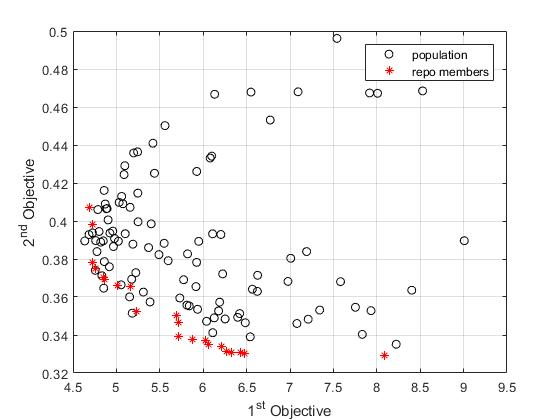
\includegraphics[scale=.6]{Fig/repo_members.jpg}
	\caption{Particles stored in external repository approximate the Pareto front.}% \textcolor{red}{This fig does not appear for some reason.}}
		\label{fig:repo_members}
	\end{figure}

Fig.\ref{fig:repo_members} presents the results of joint minimization of objective functions $o_1(\mathbf{w})$ and $o_2(\mathbf{w})$. This figure demonstrates that the repository members are Pareto optimal compared to the other particles. This figure also confirms that the repository members converge to a uniform Pareto front. 

Using the concept of Pareto optimality, we demonstrate the impact of applying kernel functions in this spatial reshaping problem by comparing the \textcolor{black}{Pareto front of the optimization problem obtained by using MOPSO} for two different scenarios including i) the optimized coefficients for the original data sample, (i.e. a linear identity function) and ii) the transformed samples under polynomial kernel whose coefficients are optimized using MOPSO. Therefore, we first optimize the coefficients of the third-order polynomial kernel function, as formulated in Eq.\ref{eq5} and then optimize the coefficients of linear features in the origin feature space. The purpose of this comparison is to investigate whether or not the resulting objective functions are fundamentally improved by incorporating nonlinear terms into the feature vectors through the proposed polynomial function.  %A two-dimension curve formed by repository members t will be drawn with two objective functions.

%This mapping by kernel method can be accounted as the input space reshaping, namely, new input sample space is produced using non-linear kernel bending feature space in order for a higher space symmetry. Reshaping result as indicated in diagram 4-6 can be obtained through testing the reshaping algorithm with test data and quadratic polynomial. More specifically, we can regard this kernel method as a mapping from two-dimension space   to three-dimension space. Because the data visualization is very important in the test, we don’t adopt polynomial kernel of higher degree.

As shown in Fig. \ref{fig:pareto_compare}, the estimated Pareto front of the nonlinear model using the polynomial kernel dominates the Pareto front of the original linear model. This result is expected since the transformed samples exhibit a higher degree of freedom by adding new dimension to the data in the feature space through the nonlinear mapping. 
A higher degree of freedom enables the MOPSO algorithm to tune the optimization parameters and find better solutions than the best solutions achievable by the original data samples. In other words, the kernel method combined with multi-objective particle swarm optimization algorithm can improve the spatial structure of the clusters quantified by the two objective functions.

%\subsubsection{Pareto Front}
\begin{figure}[t]
\centering
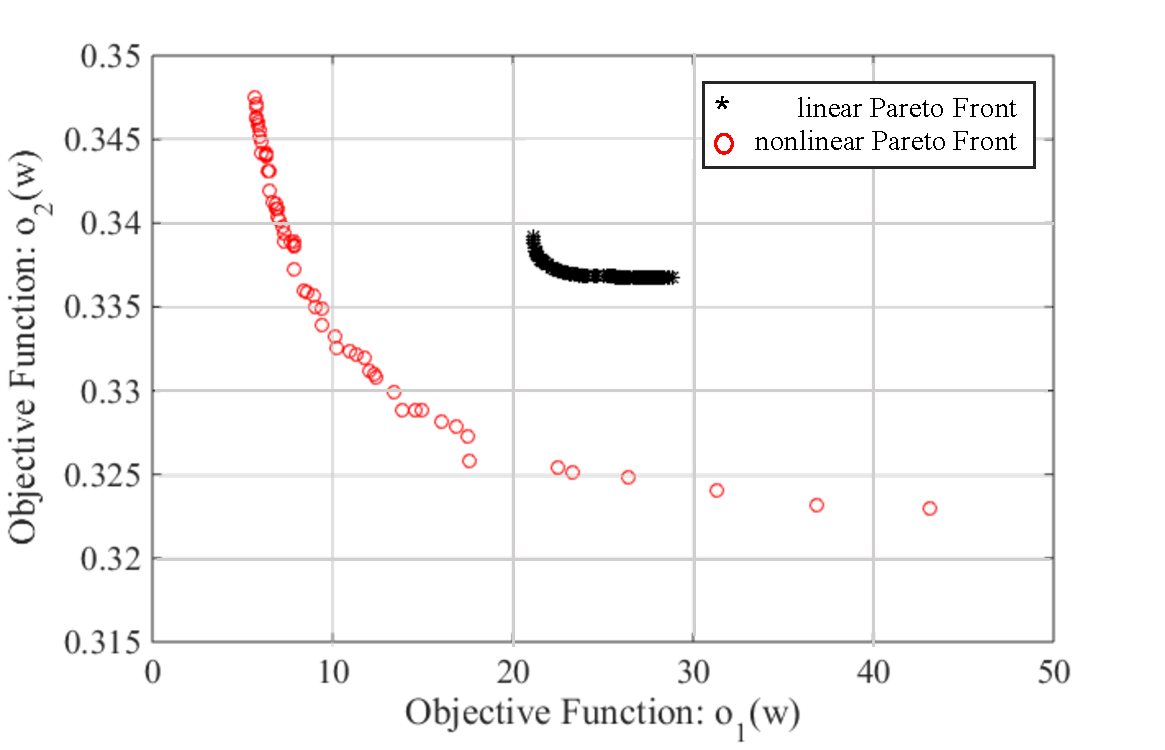
\includegraphics[scale=.6]{Fig/pareto_compare.pdf}
\caption{The \textit{Pareto front} of the results of MOPSO is significantly shifted when using the transformed feature vectors. This improvement is due to the increase in the degree of freedom provided by additional non-linear dimensions added to the samples.}
\label{fig:pareto_compare}
\end{figure}

\section{Experimental Results}\label{sec:result1}

%This section will introduce the experimental result of the aforementioned kernel-based method on test set DS2 of MITDB to show the performance. 
As mentioned in Section \ref{sec:ecgprocessing}, a cardiac segment is represented by an 8-dimensional vector $\mathbf{x}=[x_1,x_2,\dots,x_8]$ after the feature extraction and the PCA-based dimension reduction stages. %In order to reduce the complexity,  we firstly map the original 22-dimensional feature vectors, representing cardiac segments, into an 8-dimensional vectors $\mathbf{x}_{8 \times 1}$ using Principal Component Analysis (PCA). 
To specify the nonlinear transformation in (\ref{eq:z}), a polynomial function of order $3$ is applied to the feature vectors.
The resulting transformed vectors \textcolor{black}{as follows:}
\begin{align}
	[x_1,x_2,\dots,x_8,x_1^2,x_2^2,\dots,x_8^2,x_1^3,x_2^3,\dots,x_8^3,x_1x_2,....x_6x_7x_8], 
\end{align}
which include $165$ terms, 8 of which are the original features. %165 = 11 choose 8
This high dimension may cause the classifier to trap into the overfitting problem. It also significantly increases the computational complexity of the algorithm. To solve these issues, we discard some of the induced terms and include only 8 square terms $x_i^2$, 8 cubic terms $x_i^3$, and 8 cross terms of power two $x_ix_j$ and 8 cross terms of power three $x_i x_j^2$. We randomly choose these terms after discarding the redundant cross terms. Therefore, the mapped vectors $\mathbf{z}_{32 \times 1}$ include a total of $32$ terms as follows:

\begin{align}
\label{eq:8-32}
\mathbf{z}&=\{x_i^2|i=1,2\dots 8\}\cup\{x_i^3|i=1,2\dots 8\} \cup\\
\nonumber
& \{x_ix_j|i,j=1,2\dots 8,i\neq j\} \cup  \{  x_i^2x_j | i,j=1,2\dots 8,i\neq j \}
\end{align}

The performance of the aforementioned kernel-based method is tested on DS2 excluding record 232, for this record has only 7 normal samples $y_k=N$. In total, 21 records are tested.

Table \ref{table:result1} shows the performance of the proposed method in classifying ECG signal segments. In order to evaluate the consistency as well as the general classification classification results over all recordings, the median, interquartile range (IQR), mean and standard deviation of accuracy (AC), sensitivity (SE) and specificity (SP) are presented. The results are promising and the median of the classification accuracy for all classes are in the range of $88\%-99\%$. Sensitivity and specificity of the proposed method exhibit similar ranges. The mean accuracy is at least $86\%$ excluding class $V$. Therefore, this system is not likely to miss an important alarm or to report false alarms. 

\begin{table}[t]
	\caption{Classification results of the proposed method.}
	\centering
	\begin{tabular}{|c|c|c|c|c|}
		\hline
		Class N & median(\%) & IQR(\%) & mean(\%)& std (\%) \\ 
		\hline 
		AC & 94.8& 19.52 & 86.62 & 18.55\\ 
		\hline 
		SE & 97.21  & 17.36 & 87.47 &19.26 \\ 
		\hline 
		class V & median(\%) & IQR(\%) & mean(\%)& std (\%) \\ 
		\hline 
		AC & 86.11 & 27.54 & 76.41 & 22.81 \\ 
		\hline 
		SP & 99.71 & 11.22 & 90.18 & 18.52 \\ 
		\hline 
		class S & median(\%) & IQR(\%) & mean(\%)& std (\%)\\ 
		\hline 
		AC & 99.28 & 2.24& 98.29&2.57 \\ 
		\hline 
		SP & 99.64& 22.17& 97.56 & 6.06\\ 
		\hline 
		class F & median(\%) & IQR(\%) & mean(\%)& std (\%) \\ 
		\hline 
		AC & 97.91 & 8.2&93.85&7.84\\ 
		\hline 
		SP & 100.00 & 0.03&99.12&3.6\\ 
		\hline 
	\end{tabular} 
	\label{table:result1}
\end{table}

%%%%%%%%%%%%555

More importantly, the predictive capability of the proposed method is worthy of evaluating, since it is unique feature provided by the proposed system. In order to quantify the posterior probability of observing an abnormal signal after a preceding yellow alarm of similar type in (\ref{eq:personal_discrim}), the number of predicted samples are counted as formulated in Eq \ref{eq:proab}:

\begin{align}
\nonumber 
&P(\hat{y}_{k+i}=X_r|\hat{y}_{k}=X_y)=\frac{\text{\# of $y_{k+i}=X$ after $\hat{y}_k=X_y$}}{\text{\# of true alarms after $\hat{y}_k=X_y$}} \\
&P(\hat{y}_{k+i}=X_r)=\frac{\text{\# of true alarm of type $X$ ($y_{k}=X$)}}{\text{\# of all true alarms}} 
\label{eq:proab}
\end{align}

The summary of results for all 21 test records is presented in Table. \ref{table:pred_kernel}. The values provided under the column \textit{Probability of next abnormality (\%)} in Table. \ref{table:pred_kernel} present the probability of having a subsequent true abnormality of all types after observing a yellow alarm of all types along with the prior probability of observing a certain type regardless of the preceding yellow alarm in the very last column. %The last 4 columns of the Table. \ref{table:pred} show the confusion matrix of the probability of having a subsequent true abnormality of all types after observing a yellow alarm of all types. It's compared with the probability of having the same type of abnormality after a secondary abnormality of its own type. 
These results confirm the predictive capability of yellow alarms as well as the scientific fact that yellow alarm are indicative of upcoming red alarms. This conjecture supported by the fact that at least some of the heart problems develop over time, although the symptoms may appear suddenly. 
 
For instance, the prior probability of observing a sample segment with abnormal types $V$, $S$, and $F$ is respectively $\frac{96}{96+29+18}=67\%$, $\frac{29}{96+29+18}=20\%$ and $\frac{18}{96+29+18}=13\%$, based on their relative frequencies in the dataset. However, the corresponding posterior probabilities after observing a yellow alarm of type $Vp$ are respectively $\frac{38}{38+11+2}=75\%$, $\frac{11}{38+11+2}=21\%$ and $\frac{2}{38+11+2}=4\%$. This means that the probability of observing a real abnormal segment of type $V$ is $75\%-67\%=8\%$ higher than its prior probability. The same trend holds for other yellow alarms as well. The results suggest a more in-depth study of the concept of yellow alarms for heart monitoring. 
We conclude this section by stating that a new methodology provided in Chapter 4 to optimize the nonlinear transformation using an analytical approach, which significantly reduces the computational cost.

\begin{table}
	\caption{Predictive power of yellow alarms: A yellow alarm increases the chance of observing a red alarm of the same type.}
	\centering
	%\resizebox{\textwidth}{!}{
	\begin{tabular}{|m{6em}| m{2em}| m{2em}| m{2em} |m{2em}| m{2em}| m{2em}| m{2em}| m{2em}|}
		\hline
		& \multicolumn{3}{p{6em}}{Count numbers of subsequent abnormality}& &\multicolumn{3}{p{6em}}{Probability of subsequent abnormality (\%)}  & \\ 
		\hline 
		Yellow Alarm & $V_y$ & $S_y$ & $F_y$ & Total & $V_y$ & $S_y$ & $F_y$ & Total \\ 
		\hline 
		True V & 38 & 23 & 35& 96 & 75 & 75 & 61 & 67 \\ 
		\hline 
		True S & 11 & 10 & 8 & 29 & 21 & 29 & 14& 20 \\ 
		\hline 
		True F & 2 & 2 & 14 & 18 & 4 & 6 & 25 & 13 \\ 
		%		\hline 
		%		Total & 4 & 20 & 0 & 24 & 100 & 100 & 100 & 100\\
		\hline 
	\end{tabular}%} 
	\label{table:pred_kernel}
\end{table}


\section{Summary of Contributions} 
%\textcolor{red}{It is usual to have a summary of contributions at the end of each chapter. Conclusions and future works should be a separate section [bit 2 or 3 pages is sufficient.}

%\textcolor{red}{Part of the text here is the repetition of the text before revision. reword this section and provide a list of contributions and concluding remarks here. The overall conclusions should be provided in a separate section}
\textcolor{black}{In this chapter, we proposed a novel method which combines kernel-based nonlinear transformation with MOPSO optimization method. With the concept of kernel method and the loss function, we implement the method using a weighted combination of base nonlinear kernels to reshape the input feature space by mapping it to a high-dimensional space. The coefficients of kernels are optimized according to two conditions, namely, maximum separation between cluster and maximum cosine similarities between abnormal clusters.} \\
\textcolor{black}{By studying kernel method as well as heuristic optimization methods based on the spatial topology optimization concept, the outcome of this chapter can be concluded as follow:\\
\begin{itemize}
	\item translate the ideal symmetric geometry of feature space into two objective functions;
	\item design a kernel-based transformation using weighted combination of base kernels;
	\item validate that nonlinear transformations are more capable of improving the spatial topology than linear transformations.
\end{itemize}}

\textcolor{black}{%The experimental shows that approximated Pareto front produced by kernel method in the objective function space is apparently optimal to the one which is produced by the linear combinations of original features. 
In order to verify the efficiency of this method, we applied the method to test ECG samples in the MIT-BIH database\cite{mitdb}. The experimental results show that the proposed method has a classification accuracy in the range of $88\%-99\%$ for different ECG records.\\
Above all, the proposed algorithm demonstrates the potential of assessing signals deviation from its patient-specific normal trend in order to indicate the upcoming abnormality classes. The predictive capacities of the system is tested with ECG signals, but the proposed method is general and applicable to similar problems beyond the ECG signal processing, studied in this work. If a biomedical signal has one base class (i.e. normal state) and several abnormal states, we can deploy the proposed method to trigger yellow alarms and predict upcoming abnormality classes.}
  

%\fbox{\textcolor{red}{Revised up to here}}
